%!TEX root = ../../thesis.tex

\section{Overview}

Before discussing the software architecture in section~\ref{sec:software_architecture}, sections \ref{sec:rich_text_approaches} through \ref{sec:las_before_software_architecture} will discuss the apporaches, principles and goals for implementing this library without HTML editing APIs.

\section{Approaches for enabling rich-text editing}
\label{sec:rich_text_approaches}

%When not using HTML editing APIs, the components and the bahavior of native text inputs must be imitated. There are various approaches to this.

%\subsection{Overlaying an element in editing mode} One way to 

This section will discuss the options to implement rich-text editing without relying (entirely) on HTML editing APIs and discuss the advantages and disadvantages of each method. % Diese Art zu schreiben sollte der Style der Arbeit sein.

\subsection{Native input elements} Native text inputs are hard-wired to plain-text editing. No major browser offers an API for formatting. There is also no option to write HTML to an input and have it display it as rich-text. \texttt{input} fields and \texttt{textarea} elements will simply display the HTML as source code. Rich-text can only be implemented as an editable part of the website.

\subsection{Image elements} In February 2015, Flipboard Inc. demonstrated an unprecedented technique to achieve fluid full-screen animations with 60 frames per second on their mobile website\footnote{\url{http://engineering.flipboard.com/2015/02/mobile-web/}, last checked on 07/24/2015}. Instead of using the DOM to display their contents, the entire website was rendered to a \texttt{canvas} element. When a user swiped over the website the canvas element was rerendered, essentially imitating the browser's rendering engine. \texttt{canvas} elements allow rendering rich-text too. A rich-text editor can be implemented using this technique. This however has two major downsides. On the one hand it would require implementing a text-rendering engine. The \texttt{canvas} API is only capable of displaying unlayouted text with specifically set line breaks. On the other hand, making the editor accessible to other developers would be much more complex since the text only exists in an internal representaion inside the editor and would not be exposed as DOM component on the website.

An approach related to rendering the text on a \texttt{canvas} element is to render the text inside a Scalable Vector Graphic (SVG). In contrast to \texttt{canvas} elements, SVGs contain DOM nodes that can be accesed from the outside. However this has no benefit over using HTML DOM nodes with the downside that SVG too has no native implementation for controlling the text flow.

\subsection{Enabling editing mode without using its API} One way to enable editing but avoiding many bugs and browser inonstistencies, is to enable the editing mode on an element, but avoid using \texttt{execCommand} to format the text. The latter could be implemented using the DOM core APIs. This would provide the user with all basic editing functions, i.e. a caret, text input, mouse interaction and clipboard capabilites. All of this would be taken care of by the browser.

This sem-radical approach would solve the problem of buggy and inconsistent \texttt{execCommand} implementations but not the problems that arise with different browser behavior on the user's text input---for instance when entering a line break. If the markup is customly generated with JavaScript, the input may break elements or simply get stuck. This was one of the reasons why Google decided to abandon editing APIs entirely\footnote{\url{http://googledrive.blogspot.fr/2010/05/whats-different-about-new-google-docs.html}, last checked on 07/21/2015}. It could be the source to many bugs, have the development of the library be dependent on browser development and ultimatively restrict the editors capabilites.

\subsection{Native text input imitation} The only other option to allow the user to change the text on a website is by manually fetching the user's input and manipulating the DOM with JavaScript. However, this does not suffice to provide the experience of a text input. The following components, common to text editing, must also be accounted for:
% These components will be discussed hereinafter.

%, major browsers offer no way to place a caret

% Only native text input components and elements in editing mode
% ''ACE'' and ''CodeMirror'' demonstrate an effective way to imitate a text input. 

 %''ACE'' and ''CodeMirror'' demonstrate it is possible to imitate a text input by composing various DOM ele
\paragraph{Caret} The most obvious part is probably the text caret. Even if a user types on his or her keyboard, a caret must be seen on the screen to know where the input will be inserted. The caret also needs to be responsive to the user's interaction. In particular, the user must be able to click anywhere in the editable text and use the arrow keys to move it (possibly using modifier keys, which's behaviour even depends on the operating system used).

\paragraph{Selection} Just like the caret, the user must be able to draw a text selection using his or her mouse and change the selection using shift and the arrow keys. Most systems allow double clicks to select words and sometimes tripple clicks to select entire paragraphs. Other systems, for example OS X, allow holding the option key to draw are rectengular text selection, independent of line breaks.

\paragraph{Context menu} The context menu is different in text inputs from other elements on a website. Most importantly, it offers an option to paste text, that is only available in native text inputs or elements in editing mode.

\paragraph{Keyboard shortcuts} Text inputs usually allow keyboard shortcuts to format the text and to perform clipboard operations. Formatting the text is possible through DOM manipulation, pasting text however natively only works on text inputs or elements in editing mode. % is a challenge, since browsers do not offer arbitrary access to the clipboard for security reasons.

\paragraph{Undo / Redo} Undo and redo are common functions of text processing and it may be frustrating to users if they were missing.

\paragraph{Behaviour} Rich-text editors (usually) share a certain behaviour on user input. When writing a bulleted list, pressing the enter key usually creates another bulleting point instead of inserting a new line. Pressing enter inside a heading will insert a new line. However pressing enter when the caret is located at the end of a heading commonly creates a new text paragraph just after that heading. Other rules that need to be considered will be discussed in section [implementation].

\section{Approaches for imitating native components} 

These components are natively available for text inputs across all browsers. Switching an element to editing mode enables these components too. That means a user can click in a text to place a caret and move it with the keyboard's arrow keys. He or she can copy and paste text. The browser offers a native context menu that allows pasting on input elements as well as on element in editing mode. All major browsers implement a behaviour for the user' input that is common for rich-text editing (as described above).

When not using editing APIs, all of this must be implemented with JavaScript. This requires a lot of trickery and many components must be imitated to make it \textit{seem} there is an input field, where there is none. The user must be convinced he or she is using a native input and must not notice he or she is not.

\begin{figure}[!htb]
\centering
\makebox[\textwidth]{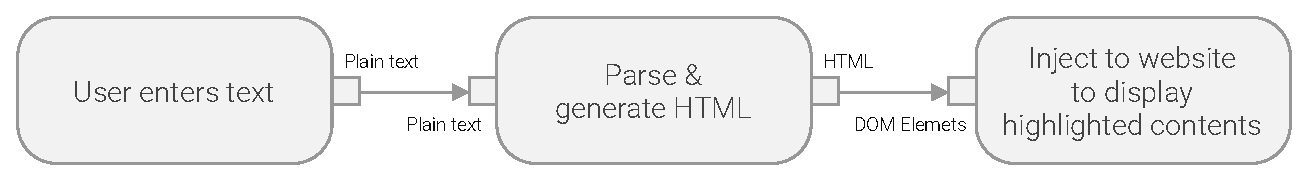
\includegraphics[width=\textwidth]{images/ace-codemirror-uml.eps}}
\caption{Rendering of highlighted source code in Ace and CodeMirror}
\label{fig:ace_rendering_uml}
\end{figure}


Web-based code editors like ''Ace'' and ''CodeMirror'' demonstrate that this is possible. They display syntax-highlighted source code editable by the user. The user seemingly writes inside the highlighted text and is also presented with a caret as well as the above mentioned components. In reality, the content inside the editor that a user sees is a regular part of the DOM---non-editable text, colored and formatted using HTML and CSS. When the user enters text, the input will be read with JavaScript. Based on the input Ace and CodeMirror generate HTML and add it to the editors contents, to show a properly syntax-highlighted representation (see figure~\ref{fig:ace_rendering_uml}). A \texttt{div} element that is styled to look like a caret is shown and moved with the user's keyboard and mouse input. The user's text input will be inserted at the according text offset. Amongst others, Ace and CodeMirror use other elements like \texttt{div}s to display a text selection and a \texttt{textarea} to fetch keyboard inputs, to recreate the behavior and capabilites of a native text input. Google's document editor uses similar techniques too.

%In reality, the user's input will be read with JavaScript and the code he or she sees is HTML generated based on this input to display syntax-highlighted text. Other components, like the caret and even the selection \texttt{div} elements, styled and positioned to mimick their native counterparts. 

%All this creates the illusion of a native text input.

%Many of the techniques to mimick a native text input like this can be found in web-based code editors like ''ACE'' or ''CodeMirror''.

Using tricks and \textit{faking} elements or behavior is common in web front end development. This applies to JavaScript as well as to CSS. For instance, long before CSS3 has been developed, techniques (often called ''hacks'') have been discussed on how to implement rounded corners without actual browser support. Only years later, this has become a standard. This not only enables features long before the creators of browsers implement them, this \textit{feedback} by the community of web developers also influences future standards. Encorporating feedback is a core philisophy of the WHATWG, the creators of HTML5.

Hacks are a necessity for an editor like this. The following sections will discuss each part of the editor and describe ideas, techniques and hacks that can be used for an effective implementation. In prior, we will discuss goals and principles that these techniques should be oriented towards as well as restrictions of browsers these techniqes must adapt to. % worst sentence ever

\section{Usage of HTML elements}

Ace, CodeMirror and Google's document editor shre similar concepts for imitating a native text input. For the caret, each of the editors create a \texttt{div} element, style it to make it look like a caret and move it when the user clicks in the text or uses his or her arrow keys. Each editor also uses \texttt{div} elements to display a text selection, styled to imitate the user's operating system's native selections. %In fact, there is hardly no alternative way

The concept to use HTML elements for the visible components of text editing is inevitable. Anything that can be seen on a website must exist in the DOM. The only deviation to this approach would be to resort a \texttt{canvas} element, as discussed above. The apporach to use HTML elements will be used for the implementation of this editor.

% Google, unlike Ace and CodeMirror displays a custom context menu. 

\section{Interaction with browser APIs}

Interaction with the browser must be well chosen. In some cases browser interaction can cause bugs and slow down performance while in some cases it can increase performance. The library should conform these rules:

\begin{enumerate} 
\item Minimize interaction with the DOM
\item Minimize interaction with unstable APIs
\item Use browser APIs if it improves performance or structure
\end{enumerate}

DOM operations can trigger a browser reflow\footnote{\url{https://developers.google.com/speed/articles/reflow}, last checked on 07/19/2015} which slows down the browser's performance. For this reason DOM operations should be avoided where possible.

Some APIs like the browser's \texttt{Range} or \texttt{Selection} interface are useful but known to be unstable. Libraries like Rangy try to tackle this by shimming parts of the interfaces. This requires complex methods and it is hard to account for possibly unknown bugs in the browsers' APIs. Ultimately this will also affect the library's file size. Instead of trying to fix native APIs, only as little as possible should be used. Instead of using possibly unstable APIs, pure JavaScript implementations should be used. Possibly unstable native APIs should only be used when it is inevitable.

Avoiding DOM operations and unstable APIs leads to a software architecture where the biggest part remains in its own business logic. Anything that can be implemented in pure JavaScript and does not cost performance or memory \textit{should} be implemented in pure JavaScript using own methods and data structues.

Facebook defined a similar goal for the user interface library React. React implements virtual DOM, an internal represenation of the actual DOM on which all operations should be performed, which in return does as little manipulation to the actual DOM as needed, to maximize performance. While the focus of this goal for this library is not solely performance, this part of it. However, there can be situations in which (even unstable) native browser methods may be faster than a JavaScript implementation. The text flow for instance should be left to the browser. There can also be cases in which a pure JavaScript implementation would be much more complex and would be at the expense of having a simple code structure. It must be decided in each particular case to use native and possible unstable APIs or a pure JavaScript implementation.

%Improving means it should be more explicit in what it does. The \texttt{bold} command of \texttt{execCommand} will manipulate the DOM to format text bold. It does not state in what how. Simple etc, what I have stated at Disadvantages of offering user interface components.

\section{Markup} 

The editor should be a ''good citizen'' in the ecosystem of other editors (see \refsubsec{subsec:noapi_dis_formatting}) and should generate valid markup, expressing a formatting semantically correct with as few tags as possible. The algorithm for creating markup must be able to work on any markup parsable by the browser and in return must generate predictable, \textit{simple} markup itself. It must not inject markup required for the internal workings of the editor\footnote{FirePad and Google' document editor inject markup for each text line, necessary for the internal functions of the editor}.


% dom operations could also be cached

\section{User interface components}

Most rich-text editors are implemented and distributed as user interface components. That means instead of only providing a library that offers methods to format the selected text and leaving the implementation of the user interface to the respective developer, most libraries are shipped as input fields with a default editor interface that is, at best, customizable.

This can be unfitting for many situations. The user interface of an editor highly depends on the software it will be integrated in. Within the software the interface may even vary depending on its specific purpose. For instance, a content management system may require an edtitor with a menubar offering many controls while a comment form on a blog requires only very little controls. Medium.com uses an interface that only shows controls when the user selects text and has no menubar at all. Assuming there are many implementations of editors that are in fact functional, it seems, choosing between editors is often just a choice of the desired ui. Customizing a ui can be just as complex as writing a ui from scratch. The latter affords to add HTML elememts and call JavaScript methods while both, customizing a user interface and writing a user interface from scratch require styling. In a worst case scenario, it can be more complex to customize an interface to specific needs then writing one from scratch and being able to define just the elements as they are required. That is why the library ''Type'' will be implemented and offered as a software library, rather than an editor and a user interface component.

%On a final note, until today, some rich-text editors use an iFrame to encapsulate the editor's contents and some don't. iFrame hat vor und nachteile. mit meiner library kann es jeder so machen, wie er/sie es will, weil es nur ne library ist.


\section{API}
\label{sec:api_design}
\label{sec:las_before_software_architecture}

\subsection{Conformity with HTML Editing APIs}

The library should be capable of any method implemented by HTML editing APIs. However the API can differ to improve they way it will be worked with.

\subsection{API Design}

% It can be much more fitting for developers to include a library that handles all text-input and -formatting operations while only providing a powerful API, leaving the ui to the developer. 

% While it can be much more fitting for developers to use an API to implement an
The API of this library must be \textit{well-designed}. That means it must be simple, effective and fit the developers' needs. The methods it offers should be simple in the sense that they conceal possibly complex tasks with understandable high-level concepts. They should be effective and fit the developers' needs in the sense that the API should be designed so that any requirement to of the developers should be matched with as little effort as possible. The API should create a workflow for developers that allows them to do what they want to do and is as easy to use and plausible as possible. jQuery is an example of encorporating an API conforming these principles.

The library's API will have two basic use cases. On the one hand, web developers must be enabled to implement rich-text editors with it. On the other hand, the library should offer interfaces for enabling web developers to extend the API and add features.

\paragraph{Extension}

For extension, web developers should have specific access to as many components and functions of the library, providing as much freedom and options as possible. This will include low-level access to components while control and explicitness is more imporant than simplicity. 

All components of Type will be implemented as classes. To provide as much capabilites as possible to other developers, all classes of Type will be exposed in a designated namespace. The classes should conform the best practices of object-oriented programming to support developers in extending the library. The class design should not only consider the specific needs of the core library but also potential use cases for other developers.

For example, with a designated class to show and move a caret, multiple carets can be instantiated for an extension that allows real-time collaboration with mutliple users. All available classes will be discussed in chapter \refchapter{ch:impl}.

\paragraph{Editor implementation}

For web developers implementing an editor (assuming the library offers all necessary features) the API should be designed to offer methods for the most common tasks related to rich text editing to allow fast and easy integration in a website. This should be high-level methods as compared to methods required for extending the library. Simplicity is more important than exact control over low-level behaviour. For implementing a rich-text editor the exposed methods should cover

\begin{enumerate}
\item Formatting and removing formats
\item Insertion
\item Deletion
\item Controlling the caret
\item Controlling the text selection
\item Controlling the clipboard
\item Controlling settings
\item Undo / redo commands
\end{enumerate}

\noindent jQuery demonstrates an effective and simple approach to API design, conforming the principles as discussed above. In jQuery all methods remain in a flat hierarchy within the root of a jQuery collection. Any method that is not a getter allows chainging and most methods are overloaded to allow passing various kinds of parameters, to determine what the function should do. Following these and the abovementioned principles, the components listed above can be expressed in 11 functions:

\begin{lstlisting}[language=JavaScript, caption=API for implementing a rich-text editor, label=lst:rich_text_api]
editor.caret([options]);
editor.selection([options]);
editor.insert([options]);
editor.format([options]);
editor.remove([options]);
editor.settings([options]);
editor.copy();
editor.cut();
editor.paste();
editor.undo();
editor.redo();
\end{lstlisting}

\noindent The functions in lines 1 through 6 can take various overloaded parameters to determine the specific action. The selection command, for instance, can be called with two numbers to draw a selection from one character offset to another (to draw a selection from characters 10 to 20 \code{editor.selection(10, 20);} can be called). It can also be called without passing parameters, to read the selection. \code{editor.selection();} would return the currently selected text as a string. A full API description can be found at table TODO.

%Applied to Type, this means

%As discussed in \refsubsec{subsec:flawed_api}, the HTML editing APIs, while being high-level and simple, still lack control and can be improved in that sense while still being simplified. As proposed in \refsubsec{subsec:adv_flawed_api}, to simplify the API and to increase control, all 17 formatting commands will be replaced with a single \code{format} method that accepts an \code{htmlString} compatible to jQuery.

%\noindent This will even account for cases where it is necessary to differenciate between an \code{i} element and an \code{em} element for semantical reasons.

\subsection{Handling use cases}
\label{subsec:api_design_handling_use_cases}

We can call programmers extending the library ''developers of the library'' and programmers using the library to implement editors ''users of the library''. To account for both use cases and maintain a clear software architecture as well as a separation of concerns, all classes that provide functionality to the library must remain in a designated namespace which the library has access to. 

\begin{figure}[!htb]
\centering
\makebox[\textwidth]{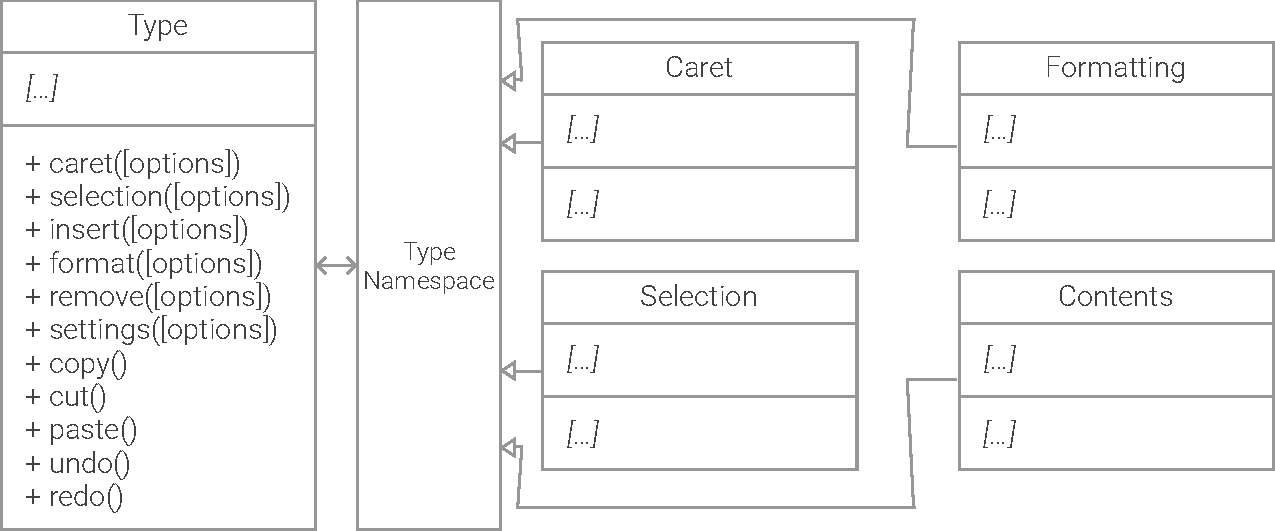
\includegraphics[width=\textwidth]{images/concept-sep-use-cases.pdf}}
\caption{Diagram of the Type library and its internally used classes (excerpt)}
\label{fig:type_uml_excerpt}
\end{figure}

The library itself will be exposed as a class to the global namespace with the name ''Type''. It can be instantiated and then provides an own API, high-level methods, for implementing a rich-text editor.

%Ursprünglich API und Codestruktur an window.execCommand orientiert, das ist aber doof.
%Bessere (weil präzisere) API mit mehr Möglichkeiten als der contentEditable scheiss
%für Programmierer und für 2 anwendungsfälle:
%einen editor bauen
%type mit plugins erweitern
%für beides gibt es die passenden Funktionen, das eine einfach und schlau, das andere präzise
%Deswegen werden auch alle Module, alle Klassen exponiert aber es gibt eine eigene API nach jQuery konzept
%Type kommt mit bestimmten Kernmodulen die fuer Textbearbeitung essenziell sind. Aber an dieser Stelle laesst sich Type um weitere Module anhand einer KOnvention (erweitern des Type Objekts) erweitern.
%Ursprünglich API und Codestruktur an window.execCommand orientiert, das ist aber doof.

%The library shall give other developers as much freedom as possible, meaning other developer should use the library as they see it fit and not the other way around, should try to conform the needs of the library.
